\section{State-of-the-art Text-To-SQL Methods}

\begin{figure}[htb]
  \centering
  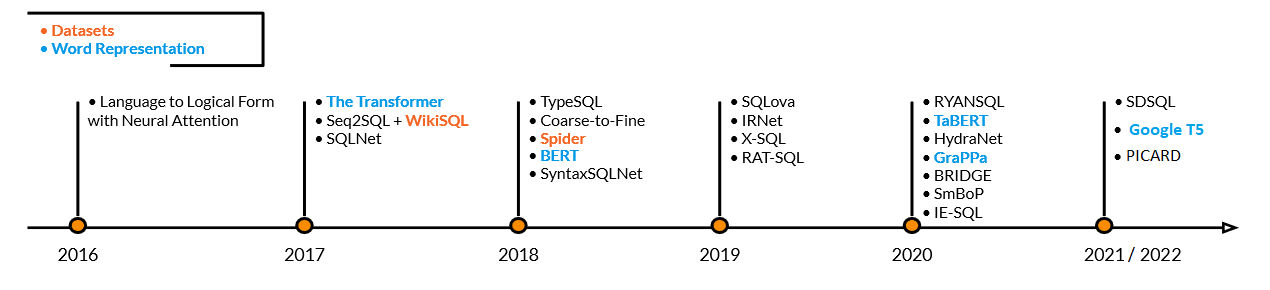
\includegraphics[width=1\textwidth]{pics/Timeline.png}
  \caption{\small Text-to-SQL over time}
  \label{fig:timeline}
\end{figure}

This section will discuss existing cross-domain state-of-the-art (SOTA), text-to-SQL models, beginning with a broad overview and moving on to individual modules. This will provide a clear picture of the progress made in text-to-SQL research. Experiments have shown that pre-trained embeddings improve models because they construct better schema linking and a more accurate SQL structure.

An efficient text-to-SQL solution requires state-of-the-art natural language processing techniques.
As a result of the neural network's capacity to take only numerical inputs and not plain text, word embedding has been used to represent numerical words.
Aside from that, in the past few years, language models have evolved to become increasingly popular as a solution for increasing performance in natural language processing tasks.
Believing that words have numerical representations that differ from others, word embeddings aim to map each word to a multidimensional vector, incorporating valuable details about the word. In addition to the brute-force creation of one-hot embeddings, researchers have developed highly efficient methods for creating representations that convey a word's meaning and relationships with other words. In most, if not all, Text-to-SQL systems, word embedding techniques such as Word2Vec\cite{DBLP:journals/corr/Rong14}, and WordPiece embeddings\cite{DBLP:journals/corr/WuSCLNMKCGMKSJL16} are used.

Recently Language models have been shown to excel at NL tasks as a new type of pre-trained neural network. It is essential to note that language models are not a substitute for word embeddings since they are neural networks and need a way to transform words into vectors.
Relying on the specific problem they want to solve, researchers can adapt the pre-trained model's inputs and outputs and train it for an additional number of epochs on their dataset. Thus, we can achieve state-of-the-art performance without complex architectures \cite{DBLP:journals/corr/abs-1810-04805}. Recent neural network architectures, like the Transformer\cite{https://doi.org/10.48550/arxiv.1706.03762}, have been used to achieve such performance by these models, which excel at handling NL and sequences of NL that are characterized by connections between words. Several language models have been used to handle the text-to-SQL task, including BERT \cite{DBLP:journals/corr/abs-1810-04805}. BERT is a pre-trained language model that has been shown to achieve state-of-the-art performance in various NLP tasks. BERT is a Transformer-based model that utilizes a bidirectional encoder to understand the representation of a word based on the context in which it appears. BERT has been used in several text-to-SQL models, such as BRIDGE \cite{lin_bridging_2020} and RAT-SQL \cite{wang_rat_sql_2021}.



% \nofootrule
\begin{figure}
    \centering
    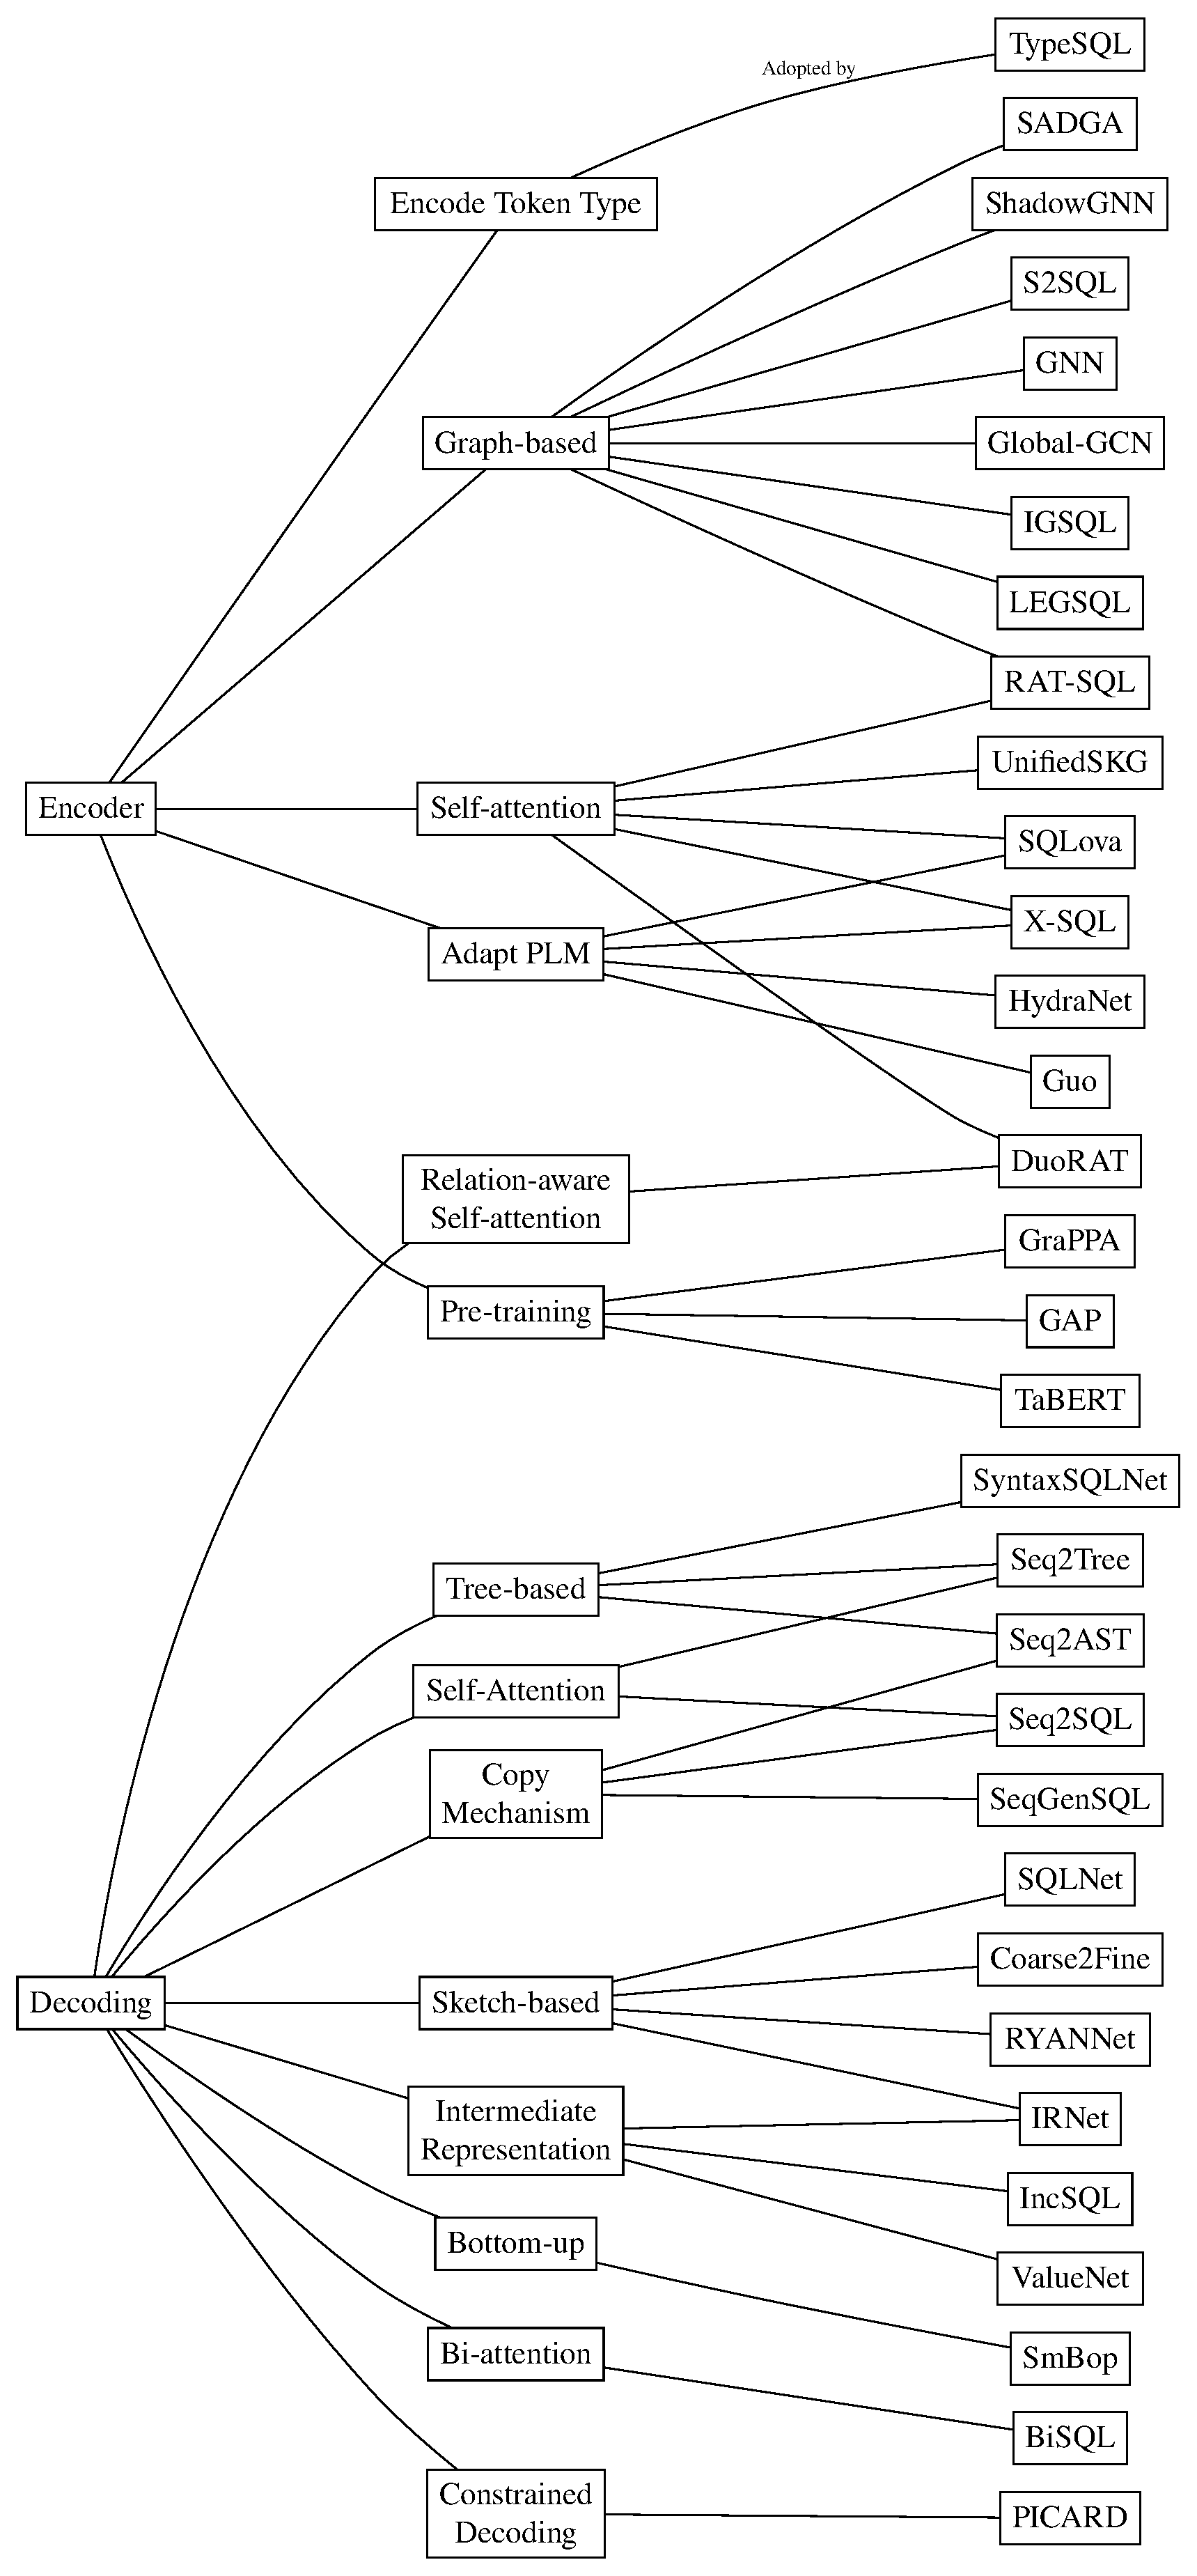
\includegraphics[height=0.98\textheight]{pics/mindmap/methods/map}
    \caption{\small{Text-to-SQL state-of-the-art Topology}}
    \label{fig:mindmap}
\end{figure}
\clearpage
\subsection{Encoding}
\label{sec:encoders}

% figure pics/transformer.jpg

\begin{figure}[H]
    \centering
    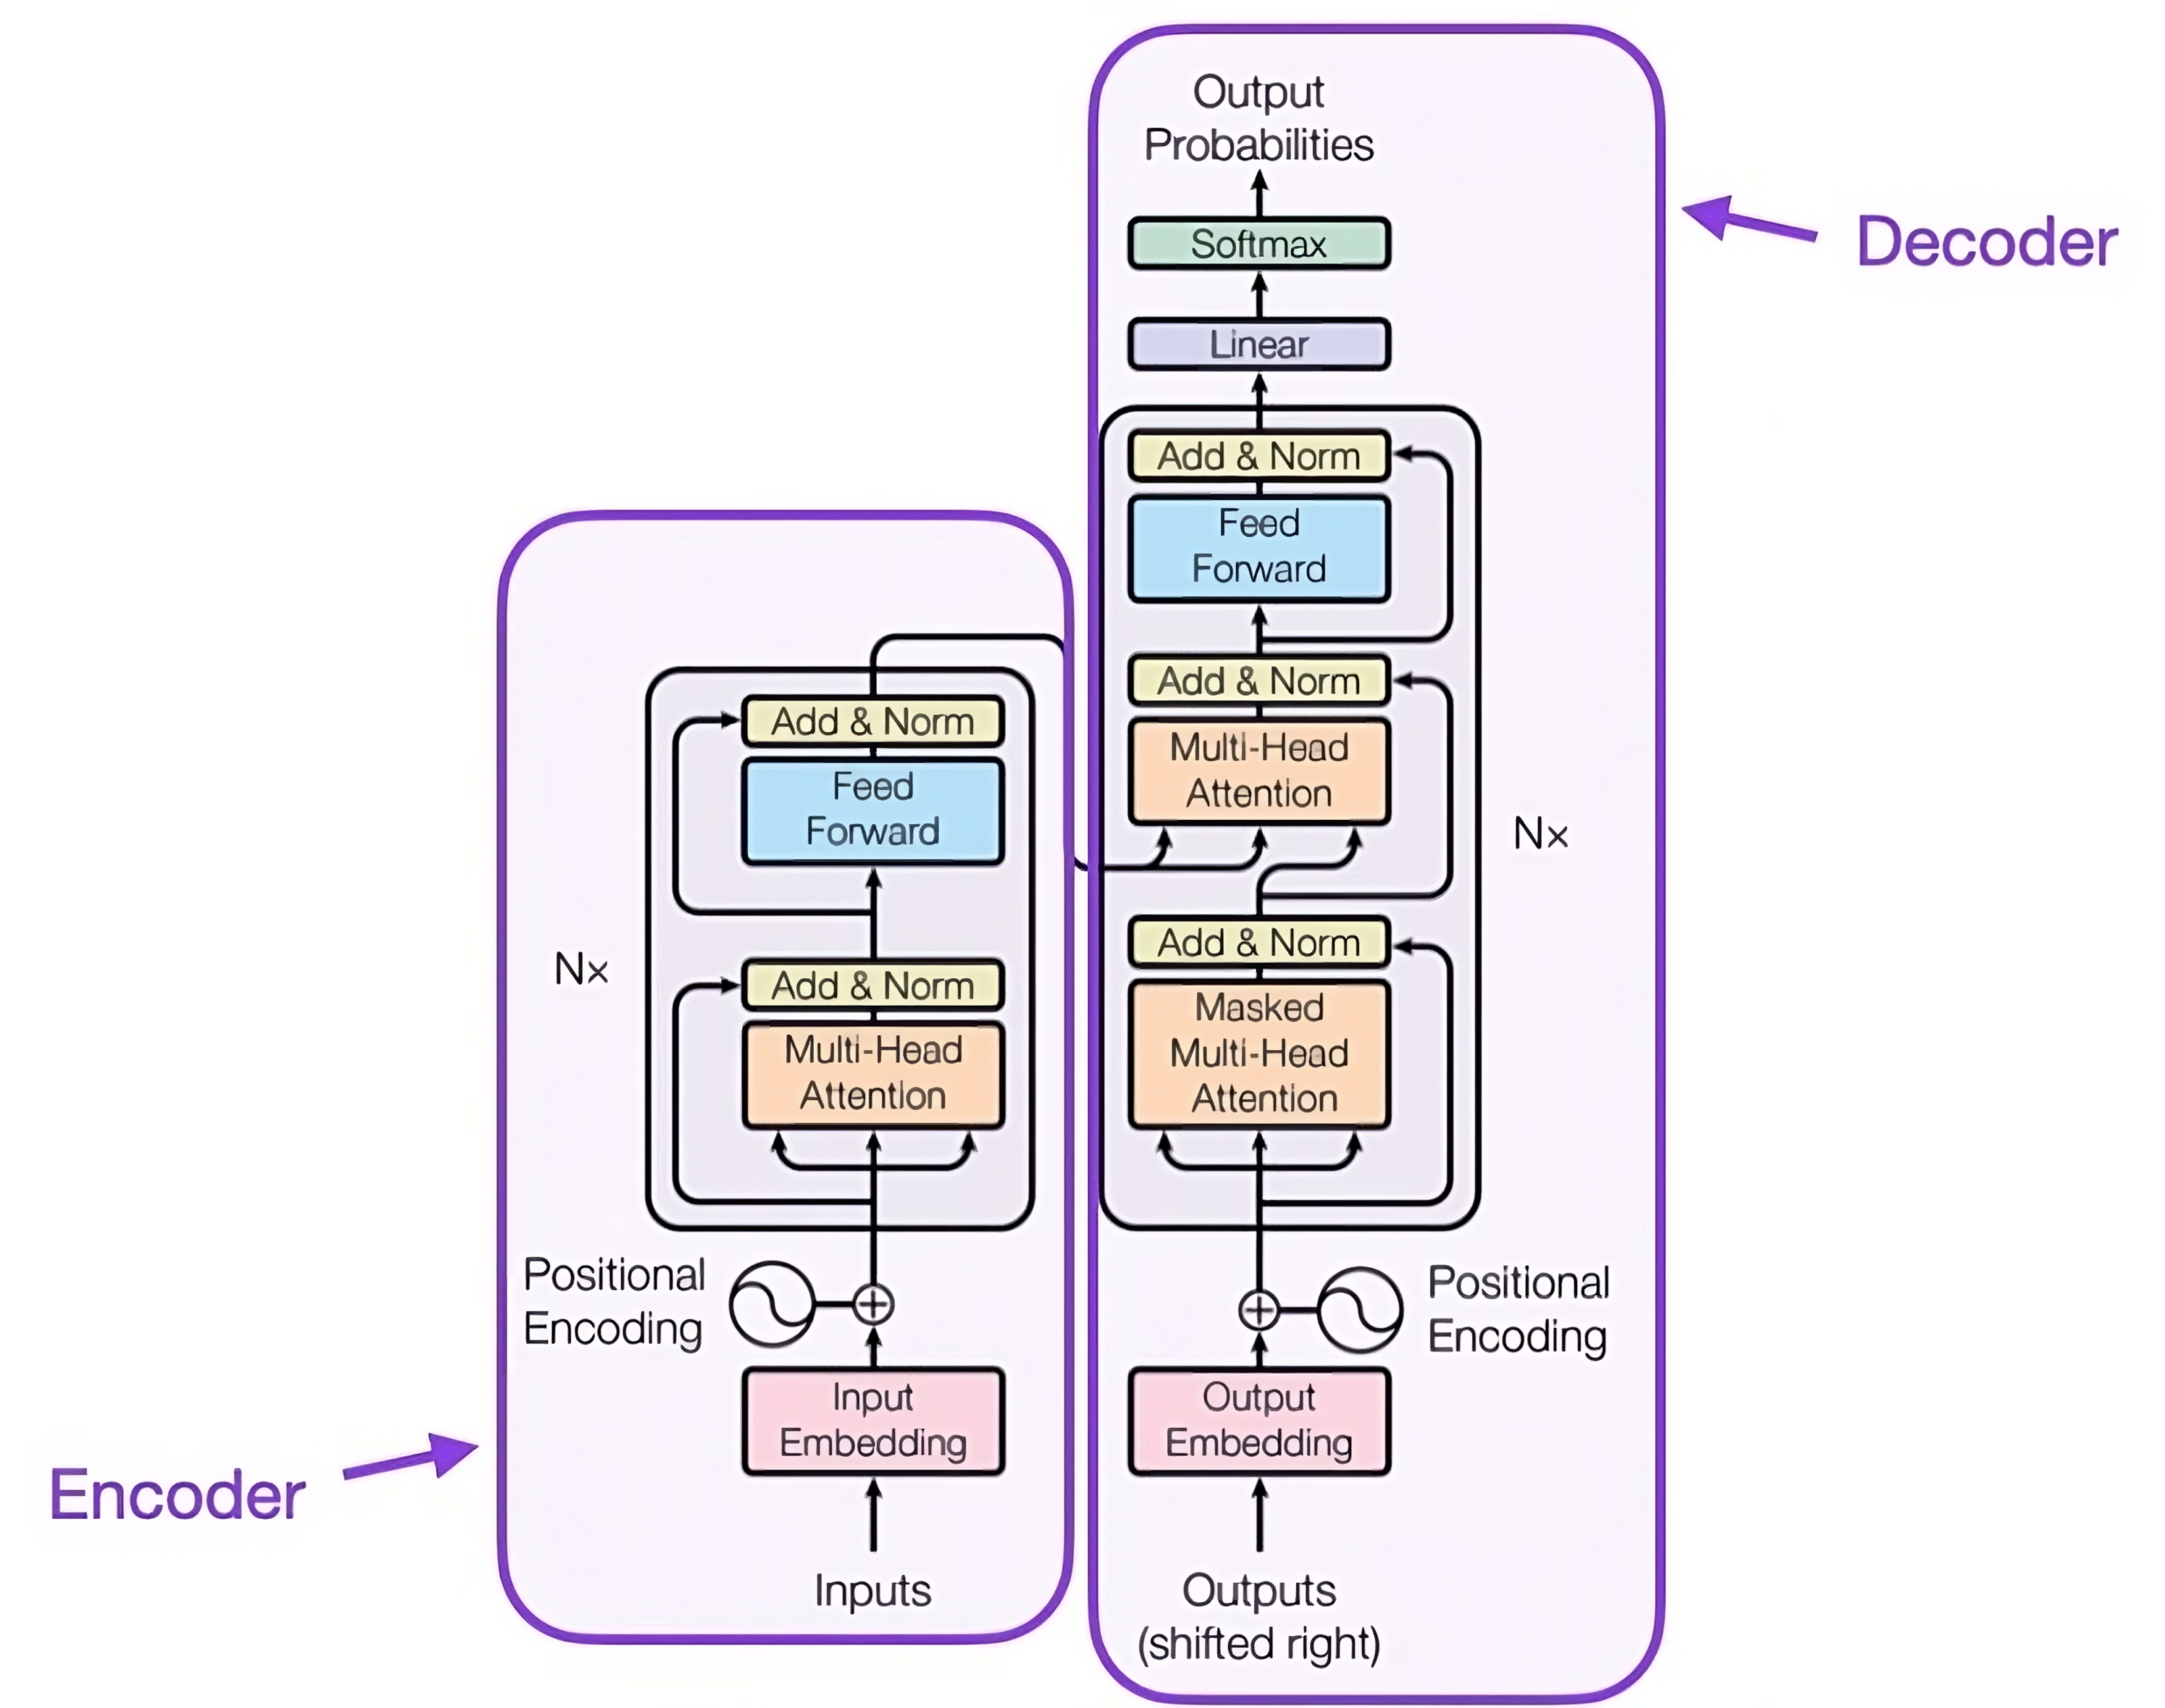
\includegraphics[width=0.8\linewidth]{pics/transformer-4x.jpg}
    \caption{Transformer architecture featured in “Attention is all you need” \cite{https://doi.org/10.48550/arxiv.1706.03762}}
    \label{fig:transformer}
\end{figure}

Encoders\cite{kumar2022deep} are a crucial component in natural language processing tasks and consist of a multi-layered assembly of recurrent elements, such as Long Short-Term Memory (LSTM) units, Gated Recurrent Units (GRUs), or other similar structures. These recurrent elements work in tandem to process an input sequence, with each unit being responsible for handling a single element within the sequence, capturing the pertinent information for that specific element, and subsequently propagating this information forward to the next recurrent unit in the stack.

The primary function of an encoder is to systematically transform textual data into a suitable numerical or vector representation that retains the inherent relationships and dependencies among words, phrases, and sentences\cite{cho-etal-2014-learning}. This is achieved through a combination of techniques, such as tokenization, embedding, and the use of attention mechanisms, which together facilitate the encoding process.

Tokenization serves to break down the input text into smaller, manageable units, such as words or subwords, while embeddings assign a dense vector representation to each token, thus allowing machines to efficiently process and compare these tokens. Attention mechanisms, on the other hand, enable encoders to weigh the importance of different input elements and selectively focus on the most relevant parts of the input sequence when generating the final encoded representation.

By effectively converting the textual data into a machine-understandable format, encoders play a pivotal role in empowering machines to recognize intricate patterns, relationships, and contextual cues within the text. Consequently, this ability to accurately discern the context of sentences and phrases forms the foundation for a wide array of natural language processing tasks, ranging from machine translation and sentiment analysis to text summarization and question-answering systems.

Several approaches have been explored to address the challenges of representing the meaning of questions, capturing the structure of database schemas, and establishing connections between database content and questions in the text-to-SQL domain\cite{deng2022recent}. These methods play a crucial role in facilitating the understanding of the complex relationships between natural language questions and their corresponding SQL queries.

One of the main challenges in text-to-SQL research is effectively representing the meaning of questions. Various encoding methods have been used to capture the semantics of natural language questions, ranging from traditional word embeddings like Word2Vec and GloVe to more advanced contextualized representations like BERT and its variants. These encoding techniques aim to produce meaningful vector representations of questions that models can use to understand and generate accurate SQL queries.

Another important aspect is representing database schemas, which serve as blueprints for organizing and structuring databases. Researchers have used various strategies to encapsulate database schema information, such as graph-based, tree-structured, and sequence-based encodings. These approaches enable text-to-SQL models to understand the hierarchical relationships and dependencies among various database elements. This allows for more accurate and efficient query generation.

Linking database content to questions is a vital task for text-to-SQL systems\cite{deng2022recent}. It involves the identification and mapping of relevant entities and attributes from the question to the database schema. To achieve this, various methods have been employed, including attention mechanisms, entity-linking techniques, and schema-agnostic encodings. These approaches help models identify relevant portions of the database schema and generate SQL queries that accurately reflect the intended meaning of the natural language questions.

Encoding methods and encoders play a crucial role in addressing the challenges of representing question semantics, encapsulating database schema structures, and linking database content to questions in the text-to-SQL domain. The exploration of diverse encoding techniques has led to significant advancements in the development of more accurate and efficient text-to-SQL models, furthering the field's understanding of the complex relationships between natural language questions and SQL queries\cite{deng2022recent}.

\begin{table}[H]
    \centering
    \newcolumntype{g}{>{\columncolor{Gray}}c}
    \begin{tabular}{|c|c|c|c|}
        \hline
        \rowcolor{Gray}
        \textbf{Methods}                & \textbf{Adopted by} & \textbf{Applied datasets} & \textbf{Addressed challenges}                                                                              \\
        \hline

        Encode token type               & TypeSQL             & WikiSQL                   & Representing question meaning                                                                              \\
        \hline
        \multirow{8}{*}{Graph-based}    & GNN                 & Spider                    & \multirow{8}{*}{\parbox{5cm}{Representing question and DB schemas in a structured way and Schema linking}} \\
                                        & Global-GCN          & Spider                    &                                                                                                            \\
                                        & IGSQL               & Sparc, CoSQL              &                                                                                                            \\
                                        & RAT-SQL             & Spider                    &                                                                                                            \\
                                        & LEGSQL              & Spider                    &                                                                                                            \\
                                        & SADGA               & Spider                    &                                                                                                            \\
                                        & ShawdowGNN          & Spider                    &                                                                                                            \\
                                        & S2SQL               & Spider                    &                                                                                                            \\
        \hline
        \multirow{5}{*}{Self-attention} & X-SQL               & WikiSQL                   & \multirow{5}{*}{\parbox{5cm}{Representing question and DB schemas in a structured way and Schema linking}} \\
                                        & SQLova              & WikiSQL                   &                                                                                                            \\
                                        & RAT-SQL             & Spider                    &                                                                                                            \\
                                        & DuoRAT              & Spider                    &                                                                                                            \\
                                        & UnifiedSKG          & WikiSQL, Spider           &                                                                                                            \\
        \hline
        \multirow{4}{*}{Adapt PLM}      & X-SQL               & WikiSQL                   & \multirow{4}{*}{\parbox{5cm}{Leveraging external data to represent question and DB schemas}}               \\
                                        & SQLova              & WikiSQL                   &                                                                                                            \\
                                        & Guo                 & WikiSQL                   &                                                                                                            \\
                                        & HydraNet            & WikiSQL                   &                                                                                                            \\
        \hline
        \multirow{3}{*}{Pre-training}   & TaBERT              & Spider                    & \multirow{3}{*}{\parbox{5cm}{Leveraging external data to represent question and DB schemas}}               \\
                                        & GraPPA              & Spider                    &                                                                                                            \\
                                        & GAP                 & Spider                    &                                                                                                            \\
        \hline
    \end{tabular}
    \caption{Methods used for encoding in text-to-SQL \cite{deng2022recent}}
    \label{tab:methods}
\end{table}

% \clearpage
\subsubsection{Encode Token Types}

\subsubsection{Graph-based Methods}

\subsubsection{Self-attention}
\label{sec:methods:encoders:SelfAttention}

Self-attention is a fundamental component in natural language processing (NLP) models, particularly those based on the Transformer architecture. It serves as the primary building block of the transformer structure, as mentioned in the works of X-SQL\cite{he2019xsql}, SQLova\cite{DBLP:journals/corr/abs-1902-01069}, and UnifiedSKG\cite{xie2022unifiedskg}. These models employ the original self-attention mechanism by default.

The self-attention mechanism allows the model to weigh and aggregate different words or tokens in a sequence based on their relative importance\cite{https://doi.org/10.48550/arxiv.1706.03762}. In essence, it helps the model to focus on the most relevant parts of a given input while processing it. This is accomplished by computing attention scores between each pair of tokens in the input, which are then used to produce a weighted sum of the input tokens. The mechanism is particularly effective in handling long-range dependencies within the text.

However, the original self-attention mechanism can be modified to cater to specific tasks or address particular challenges. One such modification is relation-aware self-attention, employed by RAT-SQL\cite{wang_rat_sql_2021} and DuoRAT\cite{scholak-etal-2021-duorat}. This variation of self-attention is designed to take advantage of the relationships between tables and columns when working with structured data.

Relation-aware self-attention extends the original self-attention by incorporating information about the structure and relations in the input data. This additional information is used to adjust the attention scores, allowing the model to focus on the most relevant relationships between different elements in the input. As a result, models equipped with relation-aware self-attention can better handle tasks involving structured data, such as SQL query generation or table-based reasoning.

% \begin{table}[t]
%     \centering
%     \scalebox{0.8}{
%         \begin{tabular}{lcc}
%             \toprule
%             \textbf{Model}                                 & \textbf{EMA Dev.} \\
%             \midrule
%             X-SQL\cite{he2019xsql}                         & 89.5              \\
%             SQLova\cite{DBLP:journals/corr/abs-1902-01069} & 87.2              \\
%             RATSQL \cite{wang_rat_sql_2021}                & 69.7              \\
%             UnifiedSKG\cite{xie2022unifiedskg}             & 72.3              \\
%             DuoRAT\cite{scholak-etal-2021-duorat}          & 75.1              \\
%             \bottomrule
%         \end{tabular}
%     }
%     \caption{The exact match accuracy on the Spider dev set.}
%     \label{table:methods:encoders:SelfAttention}
% \end{table}
\subsubsection{Adapt PLM} %Pre-trained Language Models
\label{sec:adaptplm}

\begin{figure*}[htbp]
    \centering
    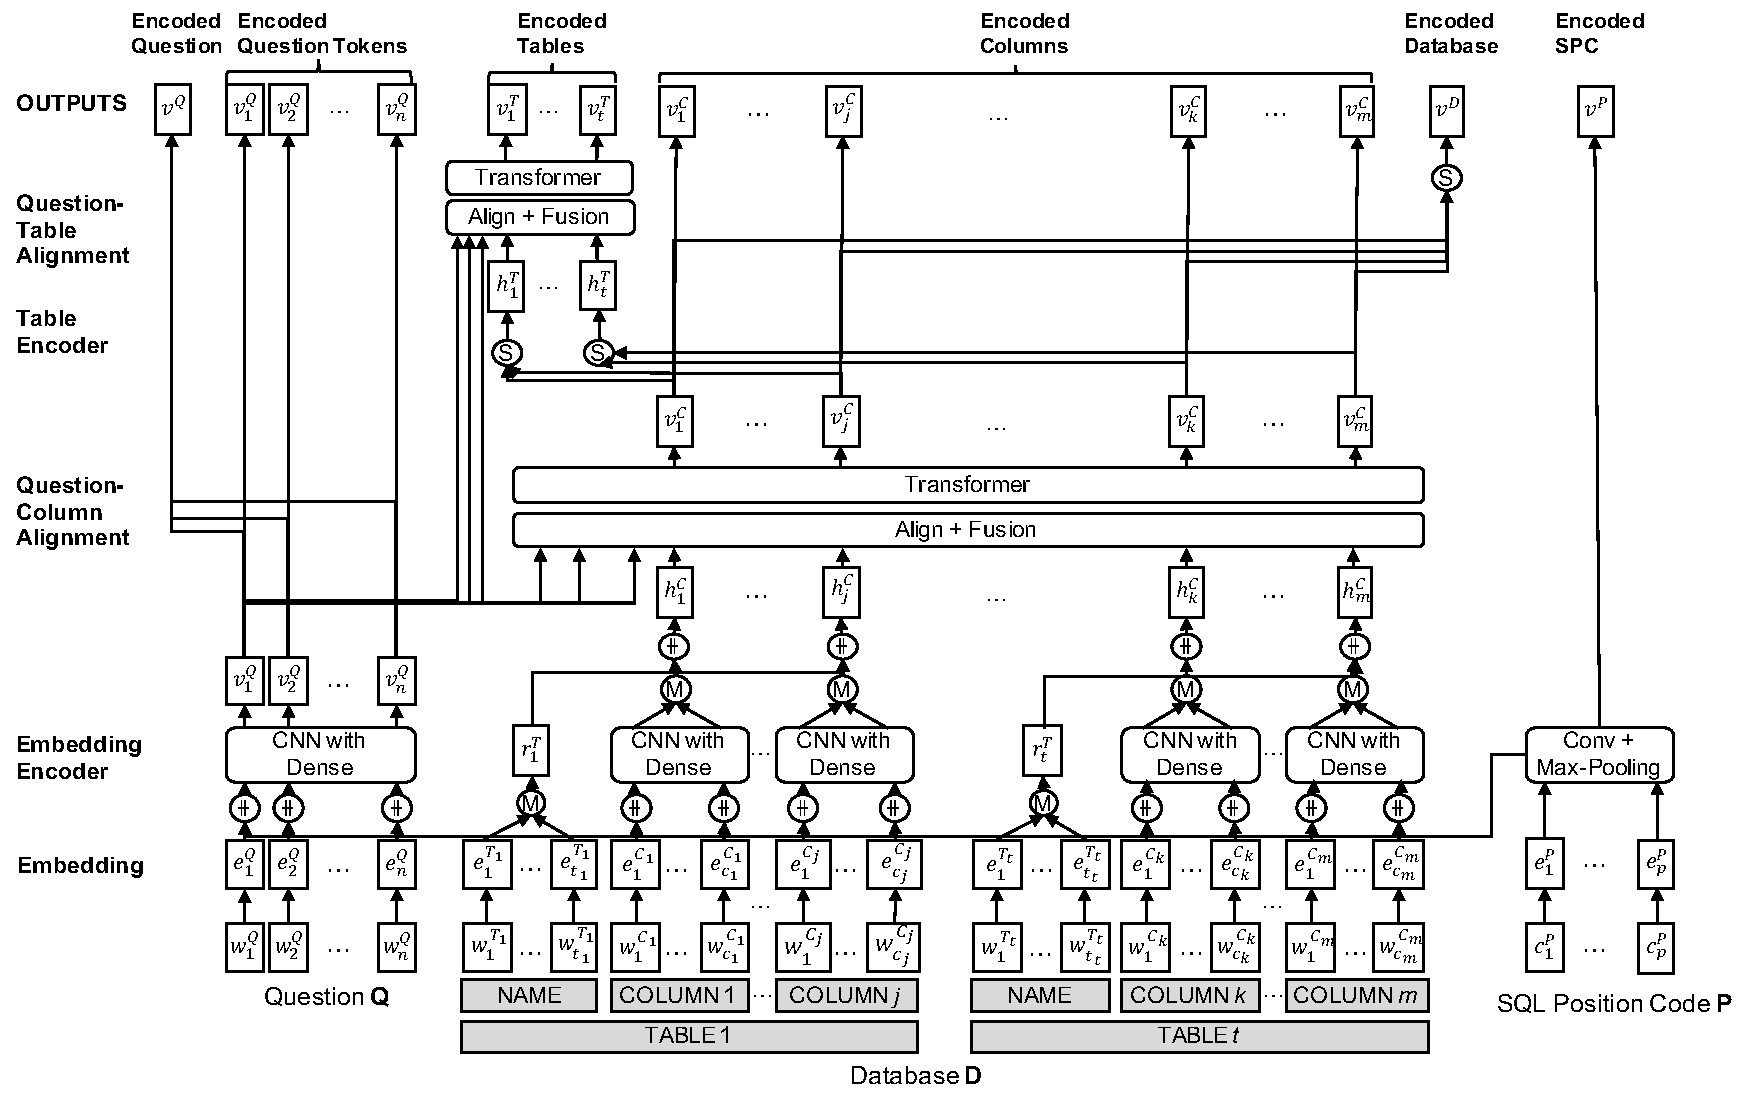
\includegraphics[width=\textwidth]{pics/enc/fig_encode}
    \caption{Network architecture of the proposed input encoder. \raisebox{-0.5ex}{
\includegraphics[height=3.3mm]{pics/enc/mark_1}} represents vector concatenation, \raisebox{-0.5ex}{
\includegraphics[height=3.3mm]{pics/enc/mark_2}} represents max-pooling and \raisebox{-0.5ex}{
\includegraphics[height=3.3mm]{pics/enc/mark_3}} represents self-attention.\cite{choi_ryansql_2020}}
    \label{fig:ryan}
\end{figure*}

Adapt \ac{PLM} methods aim to utilize the knowledge encapsulated in pre-trained language models, such as BERT\cite{DBLP:journals/corr/abs-1810-04805}, to improve their performance on text-to-SQL tasks. These methods modify or extend the original PLMs to better align with the specific requirements of the task.

One common approach is to encode both the natural language questions and the database schemas using PLMs. For instance, SQLova\cite{DBLP:journals/corr/abs-1902-01069} and RYANSQL\cite{10.1162/coli_a_00403} concatenate the question words and schema words as input to the BERT encoder. This approach allows the model to learn representations that capture the relationships between questions and the underlying schema. In figure \ref{fig:ryan}, the authors of RYANSQL\cite{10.1162/coli_a_00403} propose a novel encoder that combines the BERT encoder with a self-attention mechanism to capture the interactions between the question and schema words. As you can see it passes the question words and database tables schemas through embedding layers, then concatenates them and passes them through the BERT encoder. The output of the BERT encoder is then passed through a self-attention layer to capture the interactions between the question and schema words. The self-attention layer is then concatenated with the BERT encoder output and passed through a feed-forward network to produce the final representation of the question and schema.

Some methods go a step further by adjusting the embeddings produced by the PLMs. X-SQL\cite{he2019xsql} proposes the replacement of the segment embeddings from the pre-trained encoder with column-type embeddings for the WikiSQL dataset. Guo and Gao \cite{guo2020content} introduce an approach that encodes additional feature vectors for matching between question tokens and table cells, as well as column names. These feature vectors are then concatenated with the BERT embeddings of questions and DB schemas.

HydraNet\cite{lyu_hybrid_2020} uses BERT to encode the question and individual columns, an approach that is more aligned with the tasks BERT is pre-trained on. After obtaining BERT representations for all columns, the model selects the top-ranked columns for SQL prediction


\begin{table}[t]
    \centering
    \scalebox{0.8}{
        \begin{tabular}{lcc}
            \toprule
            \textbf{Model}                                  & \textbf{Execution Accuracy} \\
            Seq2SQL\cite{zhong_seq2sql_2017}                & 60.8                        \\
            TypeSQL\cite{DBLP:journals/corr/abs-1804-09769} & 74.5                        \\
            \midrule
            SQLova\cite{DBLP:journals/corr/abs-1902-01069}  & 90.2                        \\
            Guo\cite{guo2020content}                        & 91.1                        \\
            HydraNet\cite{lyu_hybrid_2020}                  & 92.4                        \\
            \bottomrule
        \end{tabular}
    }
    \caption{The execution accuracy on the WikiSQL dev set.}
    \label{table:methods:encoders:adaptplm}
\end{table}

Examining the WikiSQL benchmark results in Table \ref{table:methods:encoders:adaptplm}, we can observe a significant overall performance improvement when employing pre-trained language models (PLMs) compared to previous methods. This enhancement can be attributed to the ability of PLMs, such as BERT, to capture complex linguistic patterns and relationships within the input data. By leveraging the knowledge encapsulated in these models and adapting them to the text-to-SQL task, researchers have been able to achieve better alignment with the specific requirements of the problem domain. As a result, PLM-based approaches have demonstrated superior performance in generating accurate SQL queries from natural language questions, surpassing traditional methods and showcasing the potential of PLMs in addressing complex language understanding tasks.

\subsubsection{Pre-training}



\clearpage
\subsection{Decoding}

Decoders \cite{cho-etal-2014-learning} form an integral part of sequence-to-sequence models in natural language processing tasks, and they are constructed as a multi-layered architecture of recurrent elements, such as Long Short-Term Memory (LSTM) units, Gated Recurrent Units (GRUs), or other analogous structures. The primary responsibility of a decoder is to generate an output sequence by predicting an output, denoted as y, for each time step. This output sequence can be a series of words, phrases, or even entire sentences, depending on the specific problem being addressed.

At each time step, the current recurrent unit within the decoder receives a hidden state from the preceding recurrent unit. This hidden state encapsulates the information gathered up to that point and serves as a vital input for the current recurrent unit to make an informed prediction. Moreover, decoders can also incorporate attention mechanisms to help focus on the most relevant parts of the input sequence when generating the output. This is particularly useful in tasks that require the decoder to selectively attend to different input elements during the decoding process.

Decoders are commonly employed in a wide range of natural language processing applications \cite{kumar2022deep}, including but not limited to, machine translation, text summarization, question-answering systems, and dialogue generation. In question-answering tasks, for instance, the output sequence generated by the decoder is often a collection of words.

Numerous approaches have been suggested to enhance the decoding process for more precise and efficient SQL generation, ultimately bridging the divide between natural language and SQL query formulation. As illustrated in the table below, we have classified these techniques into five primary categories, along with additional methodologies\cite{deng2022recent}.

\begin{table}[H]
    \centering
    \begin{tabular}{cccc}
        \hline
        \rowcolor{Gray}
        \textbf{Methods}                                           & \textbf{Adopted by} & \textbf{Applied datasets} & \textbf{Addressed challenges}                                                            \\
        \hline
        \multirow{3}{*}{Tree-based}                                & Seq2Tree            & -                         & \multirow{3}{*}{Hierarchical decoding}                                                   \\
                                                                   & Seq2AST             & -                         &                                                                                          \\
                                                                   & SyntaxSQLNet        & Spider                    &                                                                                          \\
        \hline
        \multirow{4}{*}{Sketch-based}                              & SQLNet              & WikiSQL                   & \multirow{4}{*}{Hierarchical decoding}                                                   \\
                                                                   & Coarse2Fine         & WikiSQL                   &                                                                                          \\
                                                                   & IRNet               & Spider                    &                                                                                          \\
                                                                   & RYANSQL             & Spider                    &                                                                                          \\
        \hline
        Bottom-up                                                  & SmBop               & Spider                    & Hierarchical decoding                                                                    \\
        \hline
        \multirow{2}{*}{Self-Attention}                            & Seq2Tree            & -                         & \multirow{2}{*}{ Synthesizing information}                                               \\
                                                                   & Seq2SQL             & WikiSQL                   &                                                                                          \\
        \hline
        Bi-attention                                               & BiSQL               & Spider                    & Synthesizing information                                                                 \\
        \hline
        \parbox{3cm}{Relation-aware Self-attention}                & DuoRAT              & Spider                    & Synthesizing information                                                                 \\
        \hline
        \multirow{3}{*}{Copy Mechanism}                            & Seq2AST             & -                         & \multirow{3}{*}{ Synthesizing information}                                               \\
                                                                   & Seq2SQL             & WikiSQL                   &                                                                                          \\
                                                                   & SeqGenSQL           & WikiSQL                   &                                                                                          \\
        \hline
        \multirow{3}{*}{\parbox{3cm}{Intermediate Representation}} & IncSQL              & WikiSQL                   & \multirow{3}{*}{{\parbox{5cm}{Bridging the gap between natural language and SQL query}}} \\
                                                                   & IRNet               & WikiSQL                   &                                                                                          \\
                                                                   & ValueNet            & Spider                    &                                                                                          \\
        \hline
        Constrained decoding                                       & PICARD              & Spider                    & Fine-grained decoding                                                                    \\
        % \hline
        % Execution-guided                                           & SQLova              & WikiSQL                   & Fine-grained decoding                                                                    \\
        % \hline
        % Separate submodule                                         & SQLNet              & WikiSQL                   & Easier decoding                                                                          \\
        % \hline
        % BPE                                                        & BPESQL              & Advising, ATIS
        %    & Easier decoding
        % \\
        \hline
    \end{tabular}
    \caption{Methods used for decoding in text-to-SQL \cite{deng2022recent}}
    \label{tab:decoders}
\end{table}

% \clearpage
\subsubsection{Tree-based}

\subsubsection{Sketch-based}

Sketch-based decoders have gained attention in text-to-SQL research as an approach that simplifies the generation of SQL queries by leveraging predefined query structures, or "sketches." These sketches follow SQL grammar and allow the model to focus on filling in the slots rather than predicting the output grammar and content simultaneously.

SQLNet by Xu et al.  \cite{xu_sqlnet_2017} is an example of a sketch-based model that aligns with SQL grammar. The sketch captures dependencies between predictions, which means that the prediction for each slot is conditioned only on the slots it depends on. This approach effectively avoids issues arising from equivalent serializations of the same SQL query.

Dong and Lapata  \cite{dong-lapata-2018-coarse} further refine the sketch-based approach by decomposing the decoding process into two stages. The first decoder predicts a rough sketch, while the second decoder fills in the low-level details based on the input question and the sketch. This coarse-to-fine decoding has been adopted in other works, such as IRNet by Guo et al.  \cite{DBLP:journals/corr/abs-1905-08205}.

To handle complex SQL queries with nested structures, RYANSQL by Choi et al.  \cite{10.1162/coli_a_00403} introduces a recursive method for generating SELECT statements. This model employs sketch-based slot filling for each of the SELECT statements, enabling the generation of more intricate queries.

In summary, sketch-based decoders simplify the text-to-SQL generation process by providing predefined query structures that follow SQL grammar. This approach enables models to focus on filling in content slots, captures dependencies between predictions, and allows for the handling of complex queries with nested structures. By decomposing the decoding process into multiple stages, sketch-based decoders can efficiently translate natural language questions into accurate SQL queries.
\subsubsection{Bottom-up}

\subsubsection{Attention Mechanism}

Attention mechanism decoders play a critical role in integrating encoder-side information during the decoding process. By computing attention scores and multiplying them with hidden vectors from the encoder, a context vector is generated, which is then used to produce an output token.

Various attention structures have been employed to enhance the decoder's performance and effectively propagate the information encoded from questions and database schemas. One such example is SQLNet (Xu et al., 2017) \cite{xu_sqlnet_2017}, which introduces the concept of column attention. This technique involves using hidden states from columns and multiplying them by embeddings for the question to calculate attention scores for a given column. The attention scores are then used to help the model focus on relevant columns when generating the SQL query.

Another approach, proposed by Guo and Gao (2018) \cite{guo2020content}, incorporates bi-attention over a question and column names for SQL component selection. This method enables the model to simultaneously attend to both the question and column names, which can improve the model's ability to identify and select relevant SQL components.

Wang et al. (2019) \cite{wang-etal-2019-learning} adopt a structured attention mechanism \cite{kim2017structured} that computes marginal probabilities to fill in the slots of their generated abstract SQL queries. This approach allows the model to better capture the structure of SQL queries and enhances the overall generation process.

DuoRAT \cite{scholak-etal-2021-duorat} implements a relation-aware self-attention mechanism in both its encoder and decoder components. This attention mechanism accounts for relationships between different elements within the input data, thus improving the model's ability to comprehend and generate accurate SQL queries.

Other works, such as those by Scholak et al. PICARD (2021b) \cite{Scholak2021:PICARD} and UnifiedSKG by Xie et al. (2022) \cite{xie2022unifiedskg}, use sequence-to-sequence transformer-based models or decoder-only transformer-based models that incorporate the self-attention mechanism by default. The self-attention mechanism allows the model to weigh the significance of each input token concerning other tokens in the sequence, which can enhance the quality and coherence of the generated output.

In summary, attention mechanism decoders have been an essential aspect of Text-to-SQL research, with various structures designed to improve the propagation of information and the generation of accurate SQL queries. By continuously refining and adapting these attention mechanisms, researchers aim to further enhance the performance of Text-to-SQL models.
\subsubsection{Copy Mechanism}

\subsubsection{Intermediate Representations}

Intermediate representations (IRs) are employed in Text-to-SQL research to bridge the gap between natural language and SQL queries. By using IRs, researchers can simplify and abstract SQL queries, making it easier for models to learn and generate an accurate output.

IncSQL by Shi et al. (2018)\cite{shi2018incsql} is one such approach that defines actions for different SQL components, allowing the decoder to decode these actions instead of raw SQL queries. This method reduces the complexity of the decoding process and can improve the overall performance of the model.

IRNet by Guo et al. (2019) \cite{DBLP:journals/corr/abs-1905-08205} introduces SemQL, an intermediate representation for SQL queries designed to cover most of the challenging Spider benchmark. SemQL simplifies SQL queries by removing the JOIN ON, FROM, and GROUP BY clauses and merging the HAVING and WHERE clauses. ValueNet by Brunner and Stockinger (2021) \cite{brunner2021valuenet} builds upon SemQL by introducing SemQL 2.0, which extends the original representation to include value representation. Additionally, NatSQL by Gan et al. (2021c) \cite{gan-etal-2021-natural-sql} modifies SemQL by removing set operators, such as INTERSECT, which combine the results of two or more SELECT statements.

Suhr et al. (2020) \cite{semql} implement SemQL as a mapping from SQL to a representation with an under-specified FROM clause, which they call SQLUF. Rubin and Berant (2021) employ a relational algebra augmented with SQL operators as intermediate representations, offering another approach to simplifying SQL queries.

However, one of the main challenges with intermediate representations is that they are typically designed for specific datasets and cannot be easily adapted to others. To address this issue, Herzig et al. (2021) \cite{herzig2021unlocking} propose a more generalized intermediate representation by omitting tokens in the SQL query that do not align with any phrase in the natural language utterance.

The success of intermediate representations in Text-to-SQL tasks has inspired researchers to explore their use in other executable language domains, such as SPARQL for database systems. Works by Saparina and Osokin (2021) \cite{saparina-osokin-2021-sparqling} investigate the potential of intermediate representations for SPARQL queries.

In conclusion, intermediate representations play an essential role in Text-to-SQL research by simplifying and abstracting SQL queries, making it easier for models to learn and generate an accurate output. The exploration of various intermediate representation techniques continues to improve the performance of Text-to-SQL models and inspire advancements in other related domains.
\subsubsection{Constrained decoding}

Constrained decoding methods are employed in natural language processing tasks, such as text-to-SQL, to improve the quality of generated outputs by imposing certain constraints or utilizing auxiliary models during the decoding process. These methods aim to prevent the generation of invalid tokens, exclude non-executable partial SQL queries, or facilitate the generation of complete SQL queries.

PICARD by Scholak et al., \cite{Scholak2021:PICARD} is an example of a method that sets constraints on the decoder to avoid generating invalid tokens. Other methods, such as those proposed by Wang et al. \cite{wang2018robust} and Hwang et al. \cite{DBLP:journals/corr/abs-1902-01069}, adopt an execution-guided decoding mechanism that eliminates non-executable partial SQL queries from the output candidates.

Some approaches, like Global-GNN, Bogin et al. \cite{bogin-etal-2019-global}, use separately trained discriminative models to rerank the top-K SQL queries in the decoder's output beam. This technique allows the model to reason about complete SQL queries rather than considering each word and database schema in isolation.

Chen et al. \cite{chen-etal-2020-tale} employ a gating mechanism to select between the output sequence encoded for the question and the output sequence from the previous decoding steps at each step for SQL generation. This approach helps in generating more accurate and coherent SQL queries.

Müller and Vlachos \cite{müller2019bytepair} draw inspiration from machine translation and apply \ac{BPE} (Sennrich et al.\cite{sennrich-etal-2016-neural}) to compress SQL queries into shorter sequences, guided by AST. This technique reduces the difficulties in SQL generation, leading to improved performance in text-to-SQL tasks.


% Schema linking is a component of text-to-SQL models that helps map natural language phrases to elements of a database schema.
% Skeleton parsing is a component of text-to-SQL models that helps generate the structure of an SQL query based on a natural language question. It focuses on generating the pure skeleton of an SQL query (i.e., SQL keywords).
\clearpage
\section{Data Augmentation}
\label{sec:augmentation}



\subsection{Results}

% add SPIDER benchmark diagram image
\begin{figure}[h]
    \centering
    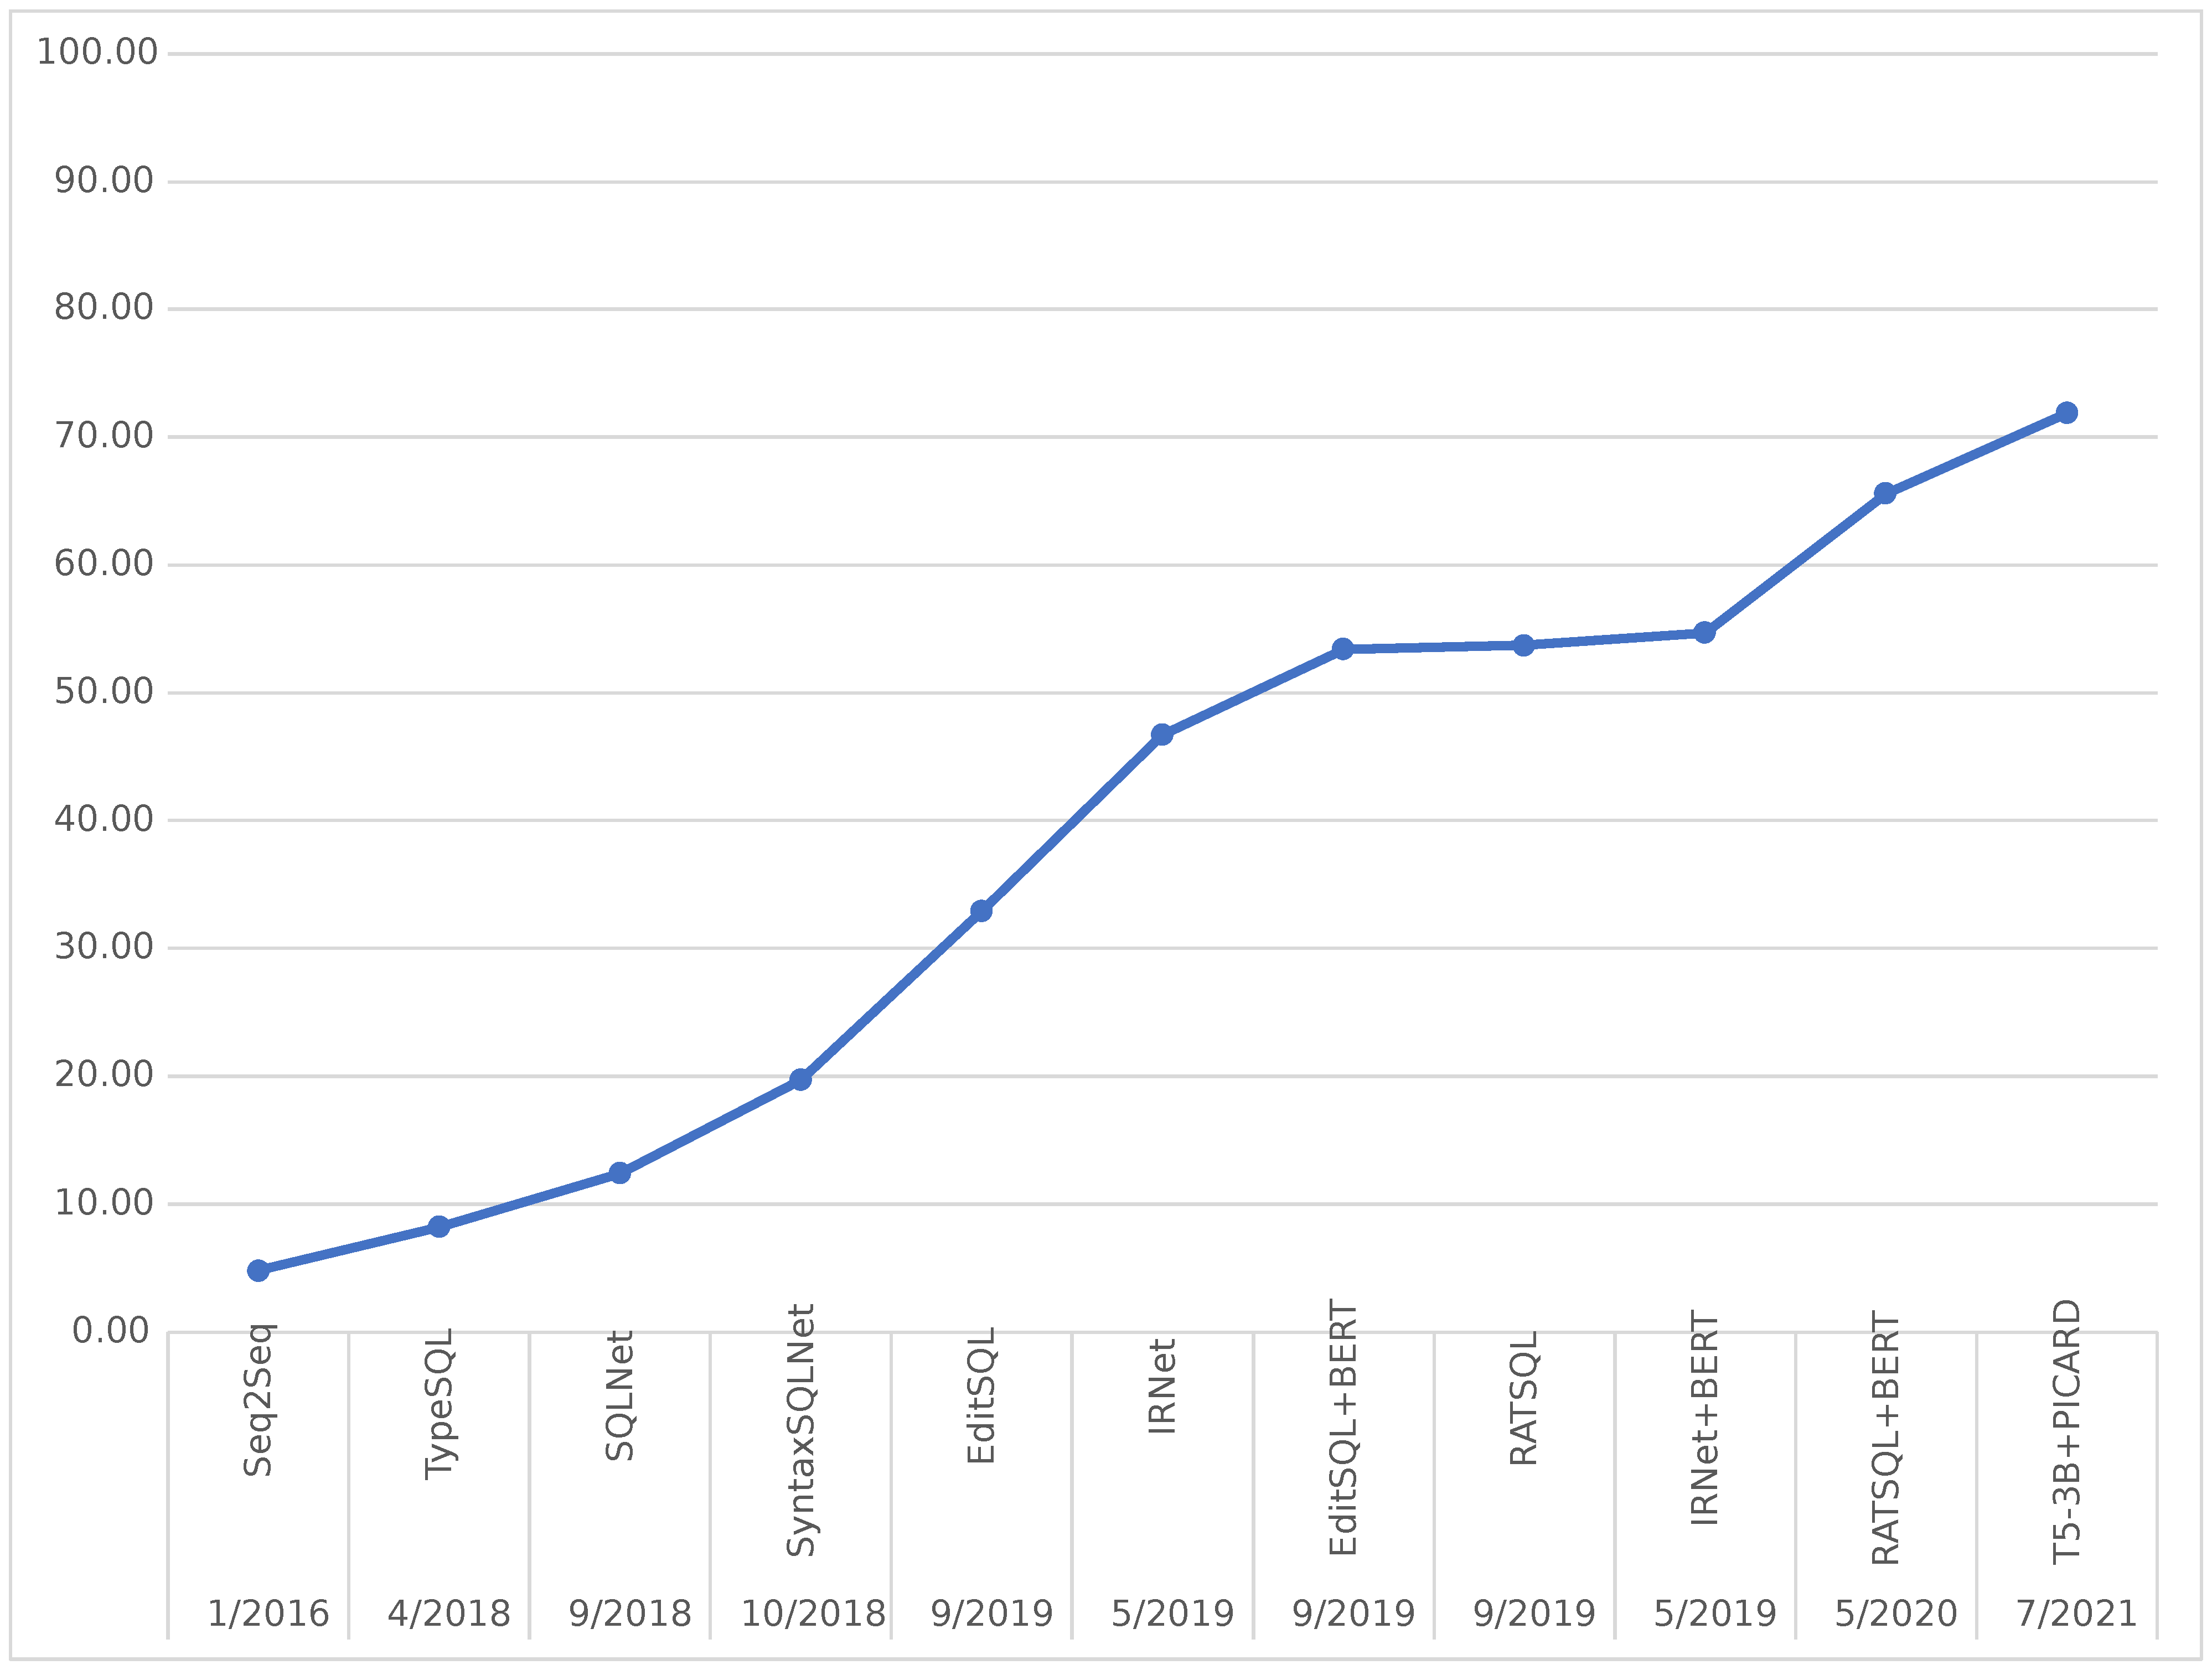
\includegraphics[width=0.99\linewidth]{pics/benchmarkeps}
    \caption{SPIDER benchmark Exact Match Results including our experiments}
    \label{fig:benchmark}
\end{figure}


Throughout this thesis, we have explored the advancements in Text-to-SQL models and their performance on the SPIDER benchmark. Our analysis revealed the significant progress made in the field, with more recent models demonstrating remarkable improvements in generating accurate SQL queries from natural language text.

The integration of powerful pre-trained language models, such as BERT, and cutting-edge architectures like T5 has played a vital role in the observed advancements. The models' ability to learn from limited labeled data, quickly adapt to new tasks or domains, and handle complex SQL queries has been substantially enhanced by employing techniques such as active learning, meta-learning, and multi-task learning.

In the following section, our experiments with ChatGPT-3.5 and ChatGPT-4.0 have showcased their superior performance, achieving scores of 81.30\% and 85.20\% on the SPIDER benchmark, respectively. These results highlight the potential of utilizing the latest huge language models for Text-to-SQL tasks, further pushing the boundaries of what is possible in this domain.

As the field of natural language processing continues to evolve, we can expect even more sophisticated models and techniques to emerge, enabling more accurate and efficient understanding and generation of SQL queries from natural language input. Future research in this area may focus on enhancing the models' ability to handle ambiguous or imprecise input, as well as exploring novel methods to improve their adaptability and generalization capabilities across diverse tasks and domains.

In the next section, we will illustrate different methods for evaluating the performance of such models.